\chapter{Learning human manipulation skill}
\label{cha4}
% Motivation - Methodology - Experiment - Result - Discussion

\section{Introduction}
\label{cha4:sec1}
% Motivation
% OM is important: what it can do? how it helps human?
In our daily life, object manipulation is one of the most commonly used skills, which includes a large category of activities ranging from the simple pick-and-place task to the complicated dexterous manipulation task like writing and using chopsticks. Service robot won't be able to really ``serve'' human without these manipulation abilities. Enabling robot to do manipulation tasks can alleviate human workload and free human from many chores. However, a robot with human level manipulation skill still only live in science fiction.

% OM is difficult: why it is difficult?
Generally, manipulation tasks are very difficult for robot. Different from pure motion planning, manipulation planning aim to not only move the robot to a desire state, but also change the environment to a desire state. Therefore in addition to robot motion planning, the impact robot put on the environment, i.e. robot environment interaction, has to be planned. The object interactions are usually complex and hard to predict as they involve complicated contact situations, and the changing kinematic and dynamic property of the environment. The complicated physics in object interactions makes manipulation tasks difficult. The multi-body interaction and the effect of friction can cause abrupt changes in the environment. This makes the environment nonlinear and non-stationary.

% What is solution to OM? - adaptive control. What is AC? Benefit of AC, but difficult to design.
Control methods depending on invariable environmental parameters is not efficient for most manipulation tasks. Adaptive control method, which focus on handling varying parameters and initial uncertainly, is required for manipulation. Adaptive control strategy is usually hard to design, especially when it involves complex environment. This demands deep inside to the task and the kinematic and dynamic property of the environment.

% learn AC from human demonstration: benefit...
To this end, we conduct a learning from human demonstration approach to gain adaptive control strategy. This approach has benefits in two-fold. First, we do not need to analytically derive the the kinematic and dynamic property of the environment in order to design the controller. Second, it provides a framework to easily program robot with a task skill. With an increasing use of robot in daily life, more and more tasks will need to be programmed. Nonlinear control methods are usually limited to narrow categories of tasks and hence needs to be done task by task. It is impractical to pre-program all such object manipulation tasks manually. Learning from human demonstration enable even non-programmers to program robots to do various of tasks quickly.

% what human do: prediction
Humans can perform these skilled tasks and adapt to the changes without difficulty. At the heart of this skill is prediction~\cite{flanagan2006control}. Studies from neuroscience suggest that human develop internal models for motor control, to predict the future state of the environment. By comparing the predictive state with the actual sensory state, the internal models monitor the progression of the tasks and launch the corresponding motor correction and motor reaction to adapt.

%To handle these situations, robots have to be equipped with a nonlinear and non-stationary control strategy, which is hard to design by analytical approaches.

% Conventional AC is difficult, use modular. benefit of modular
Inspired by this concept, we propose an approach to learn human adaptive control strategy. This adaptive control strategy is encoded with a modular model, which allows fast adaption to nonlinear and non-stationary system. Each module includes a forward model for context estimation and an inverse model for motor command generation. From multiple human demonstrations, we extract a set of strategies, each of which takes charge of one specific task context. By this method, we modularize human adaptive control strategy. Internal models (forward model and inverse model) are learnt within each modules with a representation that can be easily transfer to robot. When a robot executes a similar task, the forward models estimate the context of the task and ``contextized'' the inverse models to generate proper command that drives the object.
Each learnt control strategy is weighted by the similarity of the current task context and its corresponding context. The optimal strategy is computed as the linear combination of the weighted commands of each strategy.

The approach does not require any prior knowledge of the kinematics nor dynamics of the operation system, nor is it restricted to a specific robot platform. The control strategy is learnt on the object level and hence can be transfer from human to robot directly.
This work contributes a framework to modularize human adaptive control strategy of manipulation tasks and to transfer the learnt internal models to robot. To verify our approach, we use a \emph{Opening Bottle Caps} as an experimental. An adaptive control strategy is required here, as the friction between the bottle and the cap surfaces has multiple phases. We modularize the human control strategy in this task and implementing it on a robot to open both familiar and novel bottles.

In the next few sections, I will present our approach of learning a multiple module model of a human manipulation strategy~\ref{cha4:sec1}, detail the experimental setups~\ref{cha4:sec2} and discuss the results~\ref{cha4:sec3}.

\section{Modular approaches in manipulation}
\label{cha4:sec2}


We have briefly introduced our method in the previous section and
justified our design decisions in the light of related literature.  In
this section we present our method for modularizing human
demonstrations of manipulation tasks. Our goal is to acquire a modular
control policy for an object manipulation task from human
demonstration. To this end, we take a three-step approach:
\begin{enumerate}
\item Human demonstration of a task in several different contexts  (Section~\ref{cha4:sec2:demo}).
\item Extraction and modular decomposition of human control strategies
  for different contexts, building multiple internal models(Section~\ref{cha4:sec2:learn}).
\item Robot control using the integrated modules to compute motor
  commands (Section~\ref{cha4:sec2:control}).
\end{enumerate}

Figure~\ref{fig:overview} shows an overview of our framework.

\begin{figure}
  \centering
   \includegraphics[width=15cm]{./fig_cha4/overview3.pdf}
  \caption{ \scriptsize{System overview. Our system takes a
       three-step approach. 1) A human demonstrates a task in a
       variety of contexts. In the opening-bottle-cap experiment, the
       demonstrations are done with different bottles and caps. The
       object-level exerted forces and torque, and the the object's
       movements are used for training. 2) Clustering is run over the data from the human control
       strategies. Each cluster is then modeled as one module. 3) The
       multiple modules are integrated to compute motor commands to
       control a robot performing the same task in similar contexts}
  \label{fig:overview}
}
\label{fig:demo}
\end{figure}

\subsection{Human demonstrating tasks involving direct contact with objects}
\label{cha4:sec2:demo}


\begin{figure*}
  \centering
    \subfloat[\scriptsize{Optitrack markers attaching to a cap}] {\includegraphics[height=4cm]{./fig_cha4/marker2.jpg}}
    \subfloat[\scriptsize{Force torque sensor}] {\includegraphics[height=4cm]{./fig_cha4/Nano25-E.jpg}}
    \subfloat[\scriptsize{Texscan tactile sensors mounting to a glove}] {\includegraphics[height=4cm]{./fig_cha4/texscan2.jpg}}
    \caption{\scriptsize{Sensors used in the human demonstration of opening a bottle cap task.}}
  \label{fig:devices}
\end{figure*}

%Learning manipulation tasks is one of the main application of this approach. The physical properties of a manipulation task is hard to express analytically, and as a result the control strategy is hard to derive. Modeling expert's demonstration of strategies has been used as an alternative to the analytical solution.

The first step is to demonstrate a task to a robot. Demonstration-based learning has been extensively studied~\citep{calinon2007learning,dillmann2004teaching,kulic2012incremental}
as a promising approach for building robot
intelligence. %It is essential for the tasks that analytical expression of the system is hard to derive.
Learning manipulation tasks is one of the main application of this
approach. The physical properties of a manipulation task is hard to
express analytically, and as a result the control strategy is hard to derive. Modeling an expert's demonstration
of strategies has been used as an alternative to fully analytical
solutions.In previous studies, two major forms of demonstration are used in teaching manipulation tasks: kinematics teaching and tele-operation.

\paragraph{Kinematics teaching} ~\\
% ===== Why not kinematics approach? =====
In kinesthetic
teaching, a human directly contacts the robot and guides the robot's
movements to accomplish a
task~\citep{korkinof2013online,pais2014encoding,pastor2011skill,Miao2014}. The
trajectory of movements and contact force are recorded by the robot's
sensors.
% ===== Why not kinesthetic approach? =====
This method is simple and effective, but it is limited in the number
of controllable end effectors. %JJB is this right?
While a manipulation task usually involves multi-finger movement, a
human can only operate one finger with each hand and hence
two fingers simultaneously at most. Hence kinesthetic teaching is not feasible for demonstrating multi-finger tasks.

\paragraph{Tele-operation teaching} ~\\
To control multi-finger hands,
some researchers use
tele-operation~\citep{bernardino2013precision,kondo2008recognition,Fischer1998}.
This usually relies on data gloves or other motion-capture systems, which
sense the human hand and arm motions. The human motion is mapped to
the robot's to generate motions in the robot in real time, allowing
the robot to record its own interactions with the environment.
In fine manipulation tasks, the robot platforms are usually restricted
to anthropomorphic hands for better mapping.
Neither kinesthetic teaching nor
tele-operation method provides direct force
feedback to the human demonstrator during manipulation. With only visual feedback,
it is difficult for the human to conduct manipulation naturally.

\paragraph{Human direct demonstration} ~\\
Another approach involves the human demonstrating manipulation tasks
with their own bodies, rather than directing the
robot~\citep{asfour2008imitation}. With direct interaction with the
object, the human demonstrator is able to perform the task most
naturally and with a more delicate control strategy. However, the task
information captured from these human demonstrations must then be
transferred to robots. This involves the problem of creating a mapping
between the motions of a human and those of a robot, a problem known
as the correspondence problem \citep{Nehaniv02}.
Various methods for mapping between human and
robot have been
proposed~\citep{hueser2006learning,asfour2008imitation,do2011towards}. These may be augmented with correction by humans~\citep{calinon2007incremental,sauser2011iterative,romano2011human}
and by self-correction via learning~\citep{bidan2013robio}. In general, the effective transfer of human skills to robots skills remains a challenge.

Our proposed method derives from this last class of demonstrations.
We allow the subject to perform a manipulation task directly on an object and experience natural feedback. Our contribution is to
encode the strategy in a way that can then be
easily transferred to any robot platform. In our task demonstration, a human wears tactile sensors mounted on a dataglove, and directly
interacts with objects. In this way, human demonstrators have direct cutaneous and kinaesthetic feedback, which is desirable for good manipulation demonstration. To make the information embedded in the demonstration easily transferable to robots, the demonstration is recorded and expressed
from an object-centric viewpoint.


%============= Object Centric =============
\paragraph{Object centric representation} ~\\
The object-centric
viewpoint~\citep{okamura2000overview,jain2013improving,Miao2014}
centers the representation of the manipulation task on the manipulated object, rather than on the robot. This suggests that the goal of a manipulation task is to produce a desired
object movement rather than a robot end-effector movement. This makes sense also in the learning from human demonstration approach: humans may use different postures to accomplish a manipulation task and hence their motion or posture might be different but the effect on the object is the same. What the robot needs to imitate is the effect on the object but not the human posture.
Hence our approach takes this principle and learns a control strategy for
producing a desired object behavior. The demonstrated strategy expressed from the object perspective can then be transferred to a robot platform by converting the exerted force to robot joint torque.
With the object centric viewpoint the manipulation problem is simplified: we transfer from a problem of controlling multi-finger (multi-end-effector) and its interaction with the environment to controlling an object behavior.

Based on the object-centric principle, we collect the object's trajectory and the force driving it. We collected this data by a vision-based motion-capture system,
force-torque sensor and wearable haptic
devices. Figure.~\ref{fig:devices} shows a few of the sensors we used
in the opening-bottle-caps task. The representation of the data will be explained in Section~\ref{cha4:sec2:learn:objectlevel}


% ======= demonstrate in different context   =======
\paragraph{Demonstrations in different task contexts}  ~\\
In the demonstrations, the demonstrator performs a task a number of
times to generate enough data to reliably capture its key features.
The demonstrator also performs the task under a variety of conditions, e.g. a range of friction conditions, in order to explore how humans adapt to different task contexts. These different configurations must be chosen to cover a wide range.
For example, in a opening-bottle-cap task, the demonstration of opening
the tightest bottle within the capability of the learner is
included. These wide range demonstrations are then used to learn a
multiple module model.

\subsection{Learning a Multiple-Module Model}
\label{cha4:sec2:learn}
Here we detail our modeling method, explaining how we model the human manipulation strategy.  This requires determining the number of modules to represent a task strategy, learning the internal models for driving each
module, and determining how to integrate the output of the modules.

% Our approach: modular approach
The excellent ability of humans to manipulate different objects in different contexts and to quickly adapt to changes of context suggest that our central nervous system (CNS) maintains multiple internal models of outside environments, rather than a single internal model that adapts to new environment~\cite{neilson1985acquisition}.
Inspired by this, we take a modular approach to model the human adaptive control strategy. More specifically, we take the paradigm of MOSAIC~\cite{haruno2001mosaic} that we introduce in Section~\ref{cha2:sec3:cognitive}.

%MOSAIC
The system of MOSAIC is constituted by multiple parallel modules. Each module has three components: a forward model, an inverse model and a responsibility factor (RF). The forward model is responsible for estimating the task context in real time, and the inverse model is used to generate appropriate motor commands for the context. These two models are connected by the RF. The task context estimated by the forward model is compared with the actual current task context.
The RF of each module is computed according to the similarity between the predicted context and the actual context: the more accurate the forward model predicts, the higher the RF is (detailed in Section~\ref{cha4:sec2:control:rf}). The RF's of all modules are computed and then normalized.
The inverse models are weighed by their normalized RF. The final motor command is the linear combination of the commands generated by each inverse models. With this mechanism, the modules best predicting the current task context take most responsibility in the final motor command. Figure~\ref{fig:control} sketches the work flow of this system. %Though this model has raised concerns in the neuroscience community, it is not widely used in robot control.

We take this paradigm, and model our internal models using GMM. Training GMM with the Expectation Maximization algorithm (EM), we estimate the optimal values of the model parameters. Compared to the early work~\cite{wolpert1998multiple} which use Neural Networks and have to manually tune the variance of each forward model, GMM has the advantage of automatically computing the all the model parameters. Later work~\cite{haruno2001mosaic} fixes the hand tuning problem by modelling with a Hidden Markov Model (HMM) and optimizing the model with EM. With this method the forward models are assumed to be linear. In our approach, GMM allows a non-linear system to be modelled. Fig.~\ref{fig:control} illustrates the workflow of our approach. Compared to the switching modular method~\cite{narendra1997adaptive}, i.e. only one module will be activated and used to generate motor command, the linear combination of the modules requires a smaller number of modules to approximate the system dynamics.

In some tasks the forward model and inverse model are united into a single model~\cite{petkos2006learning}. For that particular task the action ($a_t$) taking the current task state ($s_t$) to the desired task state ($s_{t+1}$) is always unique. However, in many cases this mapping is not unique and hence the inverse model has to include extra variables in order to resolve the non-uniqueness. In our approach we build the forward and inverse models separately.
%However this model does not provide a method to find out number of models needed in tasks. %and the inverse model represented by the joint distribution will potentially produce an invalid command that average all possible solutions.

Despite the many applications and discussions of the modular approach, how to systematically modularize the control strategy presented during the human demonstration, i.e. how to determine the number of modules and build an appropriate model for each module, still remains an open problem. We tackle this problem with a data driven approach. We cluster the demonstration data with a hierarchical approach and model each cluster as a pair of forward and inverse models. This solution can be applied to modularize many manipulation tasks. A similar clustering method has been applied to group and build tree structures of human motion pattern primitives~\cite{kulic2008incremental}. To cluster the motion primitives, a high value and a low value of the cut off parameter are tested to evaluate the trade off effect between facilitating quick tree formation and introducing misclassification. In our approach, the cut off parameter is determined by the variance of the data and hence avoids this step. This provide us with a proper grouping of the data which can then generate proper motor commands for control. To the best of our knowledge, our work is the first realization of the modular approach in learning an object manipulation task with a real robot.

%
%
%Scientist has long been fascinated by human adaptive motor control ability and wondering the mechanism of it. One of the most evidently supported hypothesis is the multiple model~\cite{neilson1985acquisition}. %~\cite{haruno2001mosaic}



\subsubsection{Object centric manipulation strategy}
\label{cha4:sec2:learn:objectlevel}


As mentioned in Section~\ref{cha4:sec2:demo}, one of the challenges in imitation learning is the mapping problem, i.e. how to map the teacher's motions to the robot's motions so that they produce the same effects. This mapping becomes more difficult for object manipulation tasks, the goal of which is to deliver the object from the current state to a desired state. During this process the movement of the manipulator is bounded not only by its own kinematic constraints but also bounded by by the movement of the object. The object centric approach we use here get around this problem by directly learning the manipulated object behavior.

%It is more important to imitate how humans apply forces to achieve an object's desired movement, than to imitate the human limb movement. Therefore we take an ``object centric approach"~\cite{okamura2000overview}, where the control policy is taken from the object's perspective.

The object-centric approach means that our model encodes a force and
torque profile rather than the end effector movement trajectory.  The
imitation-learning objective here is not to find a policy for the end
effector movement but to find a policy that maps force and torque
to object movements. This policy allows the robot to efficiently
acquire new behaviors to accomplish the
task. %Different robots move differently to achieve the desired object movements.
Giving the robots' kinematics and the desired exerted force and torque
on the object, the robot joint torques can be deduced by their Jacobian
matrix~\citep{okamura2000overview}. To this end, we focus on the
force-torque-displacement tuple: $\{F,\tau,s\}$ demonstrated in the
task, where $F$ is the exerted force in all directions including the
grip force, $\tau$ is the exerted torque in all directions and $s$ is
the object displacement. In later sections, we refer $\{F,\tau\}$ as
the motor command (action) with notation $\{a\}$. In each
demonstration, a time series of the tuple is recorded.



\subsubsection{Decide number of modules}
\label{cha4:sec2:learn:cluster}

% ----------- why clustering -----------
Due to physical interactions with an object, a manipulation task
frequently encounters abrupt changes of the system dynamics, for
example transfer between statuses with no contact and with contact,
between statuses driven by static friction and by
dynamic friction. Different strategies should be used to handle
different dynamics. This motivates our multiple module
representation. Our approach is to extract strategies from multiple
demonstrations and build one module for each of the
strategies.
%During implementation, the system can quickly estimate the context by the sensory inputs and weight the modules according to their reliability and then generate a contextualized motor command.

% ---------- Cluster to find number of modules -----------
Different tasks may need a different number of modules. This number may not be easy to find. In previous studies~\cite{haruno2001mosaic,sugimoto2012emosaic}, the number of modules is defined as the number of different target objects or different phases in the task, which can be clearly distinct, such as with contact and without contact. However this is not always the case, many tasks do not have clear distinctions between different phases.
In a task involving more phases, humans may regard different phases as the same task context and handle them with the same control strategies. A recent study suggests that modularizing a control strategy by the number of objects can cause redundancy of modules~\cite{lallee2009}.

Here we propose a data-driven approach to properly define the number of modules for a given task. In the human
demonstrations, the same task is demonstrated with a few different task setups to explore how human adapt to them. The number of different strategies, i.e. modules, is found by analyzing the patterns of the force-torque-displacement tuple. Here the force and torque are the exerted force and torque on the object and the displacement is the object displacement.
We differentiate the patterns by clustering across
the force-torque-displacement tuple. Data in the same cluster is
considered to be governed by the same strategy. Hence the number of clusters
determines the number of modules.
%To this end, we should differentiate different types of strategies. The differences can be reflected from the different patterns of the force-torque-displacement tuple. We differentiate the patterns by clustering. Data in the same cluster is considered to be governed by the same strategy. The number of clusters is the number of modules and each module is encoded by one model.


% ----------- Distance Metric for clustering ------------
The goal of clustering is to separate a set of data into a few groups according to their similarities, such that the data in the same group are more similar to each other than those in different groups. This technique has very important applications in computer vision and language processing~\cite{warren2005clustering}. Numerous clustering algorithms have been proposed for different purposes.

Before clustering, we need to measure the similarities, i.e. the distances, between the data points we want to cluster. The similarity metric is user defined according to the purpose of clustering. One of the mostly used metrics is the Euclidean distance, which is used to measure the distance between two points. To measure the distance between each pair of time series, here we use the Dynamic Time Warping technique (DTW) instead ~\citep{berndt1994using}.
Dynamic time warping is suitable for measuring the similarity between two time series, which may have different speeds or durations. It warps the data in the time dimension and finds the optimal match between the time series. The similarity is computed as the average distance between the corresponding points in two series.


\paragraph{Dynamic time warping} ~\\
%%%%%%%%%% TODO: DTW explaination, citation.
Dynamic time warping is a technique for measuring the similarity between two time series, which may have different speeds or durations. It has an important application in speech recognition. For example, two people may utter the word ``hello'' at different speeds. Using DTW, one is able to tell that they are speaking the same word. This is achieved by warping the signal in the time dimension. The two time series' are ``aligned'' by finding their optimal match. The similarity is computed as the average distance between the corresponding points of the two time series. By this method, the similarity computed by DTW is independent of the variance in the time dimension. Figure~\ref{fig:alignDTW} shows an example of the alignment of two time series by DTW.

Here we make an assumption that our manipulation task is time independent, i.e. in the time scale, whenever we apply the same force we will achieve the same state. This assumption is feasible for a large range of tasks.

\begin{figure}
  \centering
  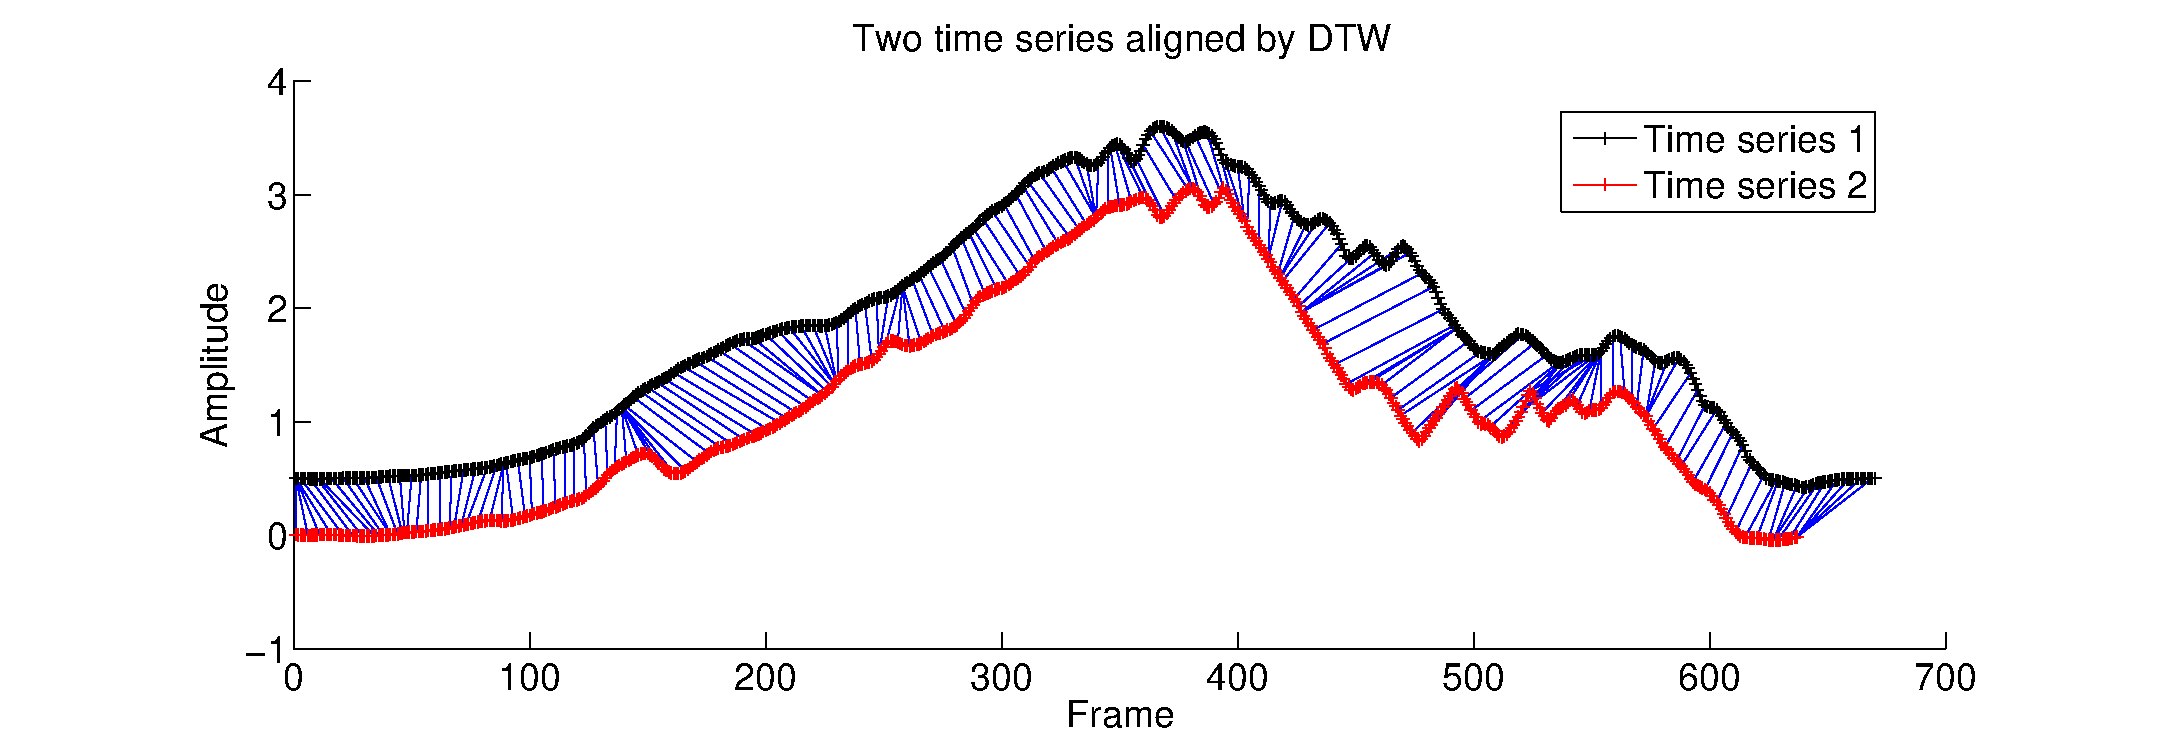
\includegraphics[width=16cm]{./fig_cha4/alignDTW.eps}
  \caption{ \scriptsize{Two time series aligned by DTW. Red and black lines are the raw time series. The blue lines connect the matching points between them. DTW wrap the two time series non-linearly so that the time independence similarity can be measured. The time series 1 is moved up by 0.5 for display reasons.}
}
\label{fig:alignDTW}
\end{figure}



\paragraph{Grouping data} ~\\
Two of the most common clustering methods are k-means clustering and hierarchical clustering. K-means is a centroid based grouping method. Given the number of clusters k, it finds a way to group the data such that the sum of the distance from each point to its belonging group center is minimized. Hierarchical clustering is a connectivity based method. There are two types of hierarchical clustering methods: agglomerative and divisive. Here we focus on the agglomerative method as it is more widely used. The hierarchical clustering method groups similar data iteratively. At the beginning each data point is a single cluster. In each iteration, two most similar clusters are merged to one. This step repeats until a stop criteria is satisfied or all data is merged to one cluster. Usually the merges are done in a greedy manner and hence no optimization is needed. Figure~\ref{fig:hcluster} illustrates the principle of hierarchical clustering. This clustering algorithm does not need to know the number of clusters in advance.

%% ------------ Hierarchical clustering -----------
In our case, the number of clusters is an unknown variable. Therefore we use the hierarchical (agglomerative) clustering method~\cite{willett1988recent} to group our data. The similarity (distance) between each pair of time series is computed by DTW. This produces a distance matrix. Each element in the matrix is the distance between two time series a and b, where a and b are the row and column index of the element. At the beginning of clustering, each time series is a single cluster. The distance between each cluster is read from the distance matrix. After one iteration, clusters are merged and most new clusters contain more than one time series. The distance between the new clusters is computed by the average distance between a member of one cluster to a member of the other cluster (average linkage).

\begin{figure}
  \centering
   \includegraphics[width=12cm]{./fig_cha4/hierarchicalclustering.pdf}
  \caption{ \scriptsize{A sketch of the hierarchical agglomerative clustering method. The nearest two clusters are grouped into one at each iteration until a single cluster is formed.}
}
\label{fig:hcluster}
\end{figure}

Our hierarchical clustering method has one more constraint: the threshold of distance. Two clusters can be merged into one only when their distance is smaller than the threshold. This threshold is set by the variance of the data from the same setup. As mentioned above (Section~\ref{cha4:sec2:demo}), a task is demonstrated a few times under the same setup. These demonstrations are presumed to be handled with the same strategy and hence belong to the same cluster. The variance of these demonstrations gives a reference of the variance of a cluster. The largest variance, across the variance of all setups, is used as the threshold for the clustering. Our clustering method is described as follow:

\begin{enumerate}
\item At the beginning, each single time series is considered to be one cluster.
\item Compute the distances between each pair of clusters.
\item Starting from the first cluster, find its nearest cluster.We define the distance between two clusters to be the average distance across all the time series pairs in each cluster.If the distance to the nearest cluster is smaller than the threshold, merge these two clusters. Otherwise leave these two separated.
\item Move to the next cluster. Repeat the last step for the rest of the clusters.
\item A new set of clusters will have been formed by the last few steps. Move to the next level of the hierarchy and repeat the step 2 to 4 until no new clusters can be formed, i.e. no pairs of clusters have distance smaller than the threshold.
\end{enumerate}

Pseudocode of the complete algorithm is shown in Algorithm~\ref{code:cluster}.

\begin{algorithm}
  \caption{Agglomerative Hierarchical Clustering}
  \begin{algorithmic}[1]
%    \Require{$x$ and $y$ are packed strings of equal length $n$}
%    \Statex Init();
    \State Init(): Make each time series a cluster; set the threshold\;
    \State $mergeable$ = true\;
    \Function{Merge}{all clusters, distance matrix} %      \Comment{$\oplus$: bit}
    \While{mergeable is true}
      \State $mergeable$ = false\;
      \For{each cluster}
        \State $ClusterA$ = current cluster\;
        \State $ClusterB$ = nearest neighbor of $ClusterA$\;
        \If{distance($ClusterA, ClusterB$) $<$ clustering threshold}
            \State Merge $ClusterB$ into $ClusterA$\;
            \State $mergeable$ = true\;
        \EndIf
      \EndFor
      %\State \Return{$\delta$}
    \EndWhile
    \EndFunction
  \end{algorithmic}
  \label{code:cluster}
\end{algorithm}

% --------- Number of cluster -----------
When the clusters cannot be merged further, we define the number of modules for this task: it is the number of the remaining
clusters. Each cluster is used as a module. The pattern of the data in a cluster represents a strategy for handling a specific task context.



\subsubsection{Learning Internal Models for Each Module}
\label{cha4:sec2:learn:model}

%%%%%%%%%%  TODO: MOSAIC
After identifying the number of modules and the data assigned to each, we build models for each module from its associated data. In this section, we explain the way we encode human manipulation strategy using machine learning to build the modules.

We aim to build a model that closely emulates the human motor strategy
in order to make the best use of the human data. Evidences of neuroscience suggest that human develop internal model for motor control, so as to estimate the outcome of a motor command. The use of internal model speed up the human correction and reaction in motor control. One hypothesis of the internal model is MOSAIC, which is a multiple modular model composed by a couple of pairs of forward model and inverse model. We build our control strategy based on this hypothesis.

\paragraph{MOSAIC} ~\\
MOSAIC~(MOdular Selection And
Identification for Control)~\citep{haruno2001mosaic} is a paradigm of multiple-module control,
where each module is composed of a forward model and an inverse
model. The forward models are responsible for estimating the task
context in real time, and the inverse models are used to generate
appropriate motor commands for the current context. The inverse models
are weighted by the accuracy of the estimations of their corresponding
forward models. The final motor command is the linear combination of
the commands factored by their weights.

We take the paradigm of MOSAIC but implement the modular model in our own manner. In earlier work, \citet{wolpert1998multiple} used
Artificial Neural Network (ANN) to encode the internal models,
i.e. the forward models and the inverse models. The variance of a
forward model, which decides how much the multiple modules
collaborate, has to be manually tuned. MOSAIC addresses this
hand-tuning problem by modeling the transition between modules using a Hidden Markov Model~(HMM) and optimizing the variance with the
Expectation Maximization~(EM) algorithm~\citep{haruno2001mosaic}. In
this method the forward models are approximated by linear systems. In order to solve the hand tuning problem of the variance but without restricting the complexity of the internal models, we encode our internal models with
Gaussian Mixture Models~(GMM)~\citep{cohn1996active}.

%During demonstrations, we constantly acquire the object displacements and the force and torque applied by the demonstrator. The demonstrator is the only source of exerted force and torque in the system. The relationship between the exerted force and torque and their resulting object displacement shows the dynamic characteristics of the task.

%GMM
\paragraph{Gaussian Mixture Model} ~\\
We model the correlation of the force and the displacement with
GMM. The task dynamics is hence encoded as a joint distribution of the object status displacement $s$ and the action $a$ taken by the human, $p(s,a,{\mid}{\Omega})$. In our experiment, $s$ is the one-dimensional angular displacement of the cap, and $a$ is the one-dimensional exerted torque and grip force.
Modeling a distribution by GMM allows us to capture the nonlinearity in the data, and also to compute the likelihood of a query data point in the model. This provides a good estimation of the reliability of the module in the current task context, which is crucial in choosing the correct modules for control  (discussed in Section~\ref{cha4:sec2:control:rf}).
Further, as a generative model GMM is able to
generate new data from the model, that is it allows us to generate motor commands. This is done by the {\em Gaussian Mixture Regression} (GMR). The general mathematical expression of GMM is explained in the previous chapter section~\ref{cha3:sec2:learn}. 

%\begin{table}
%\caption{Encoding process of GMM and computation process of GMR}
%    \colorbox{light-gray}{
%        \begin{minipage}[t]{1\textwidth}
%
%          With a Gaussian Mixture Model (GMM), the joint distribution
%          $\Omega$ of a set of variables $\{\eta\}$ is expressed as a
%          sum of $N$ Gaussian components:
%           \begin{equation}
%           \begin{split}
%            p\left(\eta\mid\Omega\right) = \sum_{n=1}^N \pi_n p\left(\eta\mid\mu_n,\Sigma_n\right) \\
%            = \sum_{n=1}^N \pi_n \frac{1}{\sqrt{\left(2\pi\right)^D \mid\Sigma_n\mid }} e^{-\frac{1}{2}\left(\eta-\mu_n\right)^{\top} \Sigma^{-1}_n \left(\eta-\mu_n\right)}
%           \end{split}
%           \end{equation}
%           where $\pi_n$ is the prior of the $n^{th}$ Gaussian component
%           and the ${\mu}_n$, ${\Sigma}_n$ the corresponding mean and
%           covariance, and $D$ the number of variables.
%
%
%            %% GMR:
%            Gaussian Mixture Regression (GMR) allows us to estimate the conditional expectation value of a variable $\eta^e$ given a query point $\eta^q$ where $\{\eta\} = \{\eta^q, \eta^e\}$. To compute this expectation value, first we define:
%            \begin{equation}
%            {
%             {\mu}_{n} = \begin{pmatrix} {\mu}_{n}^q    \\
%                                         {\mu}_{n}^e
%                         \end{pmatrix}
%            }
%%            \end{equation}
%%            \begin{equation}
%            \hspace{1cm}
%            {
%            {\Sigma}_{n} =  \begin{pmatrix} {\Sigma}_{n}^{qq}  & {\Sigma}_{n}^{qe}  \\
%                                            {\Sigma}_{n}^{eq} & {\Sigma}_{n}^{ee}
%                            \end{pmatrix}
%            }
%            \end{equation}
%
%            Secondly we compute the expected distribution of $\eta^e$ from the $n-th$ component:
%
%            \begin{equation}
%            {
%            \hat{\mu}_{n} = {\mu}_{n}^e + \Sigma_{n}^{eq}({\Sigma}_{n}^{qq})^{-1}(\eta^q-{\mu}_{n}^e)
%            }
%            \end{equation}
%
%            \begin{equation}
%            {
%            \hat{\Sigma}_{n} = {\Sigma}_{n}^{ee} - {\Sigma}_{n}^{eq}({\Sigma}_{n}^{qq})^{-1}{\Sigma}_{n}^{qe}
%            }
%            \end{equation}
%
%
%            Finally, all the $N$ Gaussian components are taken into
%            account, and the expectation value of variable $\eta^e$ is
%            computed as the mean $\hat{\mu}^e$ with the covariance
%            $\hat{\Sigma}^{ee}$:
%
%            \begin{equation}
%            {
%            \hat{\mu}^{e} = \sum_{n=1}^N{\beta_n}\hat{\mu}_{n}
%            }
%%            \end{equation}
%%            \begin{equation}
%            \hspace{1cm}
%            {
%            \hat{\Sigma}^{ee} = \sum_{n=1}^N{\beta_n}^2\hat{\Sigma}_{n}
%            }
%            \end{equation}
%
%            where
%            \begin{equation}
%            {
%            \beta_n = \frac{\pi_{n}p(q|{\mu}_{n}^q,{\Sigma}_{n}^{qq})}
%            {\sum_{n=1}^N{\pi_n}p(q|{\mu}_{n}^q,{\Sigma}_{n}^{qq})}
%            }
%            \end{equation}
%
%            Note that in a multiple module model, different module may have different number of Gaussian components.
%        \end{minipage}
%    }
%
%\label{tab:GMM}
%\end{table}



\paragraph{Internal Models}


%A forward model is held to anticipate the outcome of the motor command, while an inverse model is held to generate motor commands to take the current system state to the next state. The discrepancy between the anticipation of the forward model and the actual feedback is used to correct the motor command generated from the inverse model (Section~\ref{sec:rf}). Figure~\ref{fig:control} shows the basic control flow of a forward-inverse model pair.
As mentioned above, the internal models we are using here are the forward model and the inverse model.
A forward model is held to anticipate the outcome of the motor command, while an inverse model is held to generate motor commands to take the current system state to the next state. The discrepancy between the anticipation of the forward model and the actual feedback is used to correct the motor command generated from the inverse model (Section~\ref{cha4:sec2:control:rf}). Figure~\ref{fig:control} shows the basic control flow of a forward-inverse model pair.

\begin{figure}
  \centering
      \subfloat[\scriptsize{}]{\includegraphics[width=12cm]{./fig_cha4/control_1_2.pdf}}
      \vspace{0.5cm}
      \subfloat[\scriptsize{}]{\includegraphics[width=12cm]{./fig_cha4/control_3_2.pdf}}
      \caption{ \scriptsize{Control flow diagram of forward-inverse
          model in motor control. (a) System overview. Pairs of
          forward and inverse models work together to generate motor
          commands. The detailed mechanism inside the red box is shown
          underneath. (b) An example of a 3-module model. The forward
          models predict the current task context (s1, s2, s3) and
          estimate the accuracy of their prediction ($\lambda$1, $\lambda$2,
          $\lambda$3). These accuracy estimates are called ``Responsibility
          Factors'' as they also determine how much responsibility
          each inverse model should take in the final command. The
          inverse models generate commands (a1, a2, a3) and the final
          command is the summation of these, each weighted by its
          individual responsibility factor (a1$\lambda$1+a2$\lambda$2+a3$\lambda$3).  } }
\label{fig:control}
\end{figure}

% ----------- One model for both -------------
%The internal model ${\Omega})$ (forward model and inverse model) is encoded by the joint distributions of the variables, i.e. $p(s_t,s_{t+1},a_{t-1},a_t\mid{\Omega})$. This joint distribution encodes the forward model and the inverse model at the same time and both of their functionalities can be realized by the Gaussian Mixture Regression (GMR). For a given previous state and previous motor command, GMR provides a close-form solution to compute the anticipating state $s_t$, i.e. $p(s_{t+1}{\mid}s_{t},a_{t},{\Omega})$. For a given current state and desired state, we can compute the motor command using GMR, i.e. $p(a_t{\mid}s_t,s^{*}_{t+1},{\Omega_f})$. In some tasks, the initial status of the system remains unchanged for a certain time until the exert force or torque is big enough to change it. This will cause degeneracy in the inverse model. To solve this problem we include the previous motor command into the model, i.e. $p(a_t{\mid}s_t,s^{*}_{t+1},a_{t-1},{\Omega_f})$.

% --------- one model for each ----------
We encode the forward model $\Omega_F$ by the joint distributions of the current system state (object displacement), previous system state and the previous motor command, i.e. $p(s_t,s_{t-1},a_{t-1}\mid{\Omega_F})$, and similarly encode the inverse model $\Omega_I$ by the joint distributions of the current system state, the desired next system state, previous motor command and the current motor command, i.e. $p(s_t,s^{*}_{t+1},a_{t-1},a_t{\mid}{\Omega_I})$.
The previous motor command $a_{t-1}$ is necessary for the inverse
model. In some tasks, the system status can remains unchanged for a
certain period until the exerted force reaches a threshold to change
it. This will cause degeneracy in the inverse model; hence we
include the previous motor command in the model to tackle it.



% Non-linear, multi model. What to solve in multi model
%As discussed above, one of the characteristics of manipulation task is the changing kinematics and dynamics configuration.
%In different task contexts, the pattern of the correlation between the displacement and action may be different.

%By clustering the training data into different groups as discussed in Section~\ref{cha4:sec2:learn:cluster}, we are able to discover the number of different patterns, i.e. number of modules. We train one GMM on each of the modules to encode the different changing patterns of the task context.


% Learn system dynamics, impedance, admittance.

%Phases
%A single model is usually not enough to encode all these different configurations. Therefore we adopt a multiple modular approach to model the different environment. There are two key problems needed to be resolve in a multiple modular approach: how many models to build (Section~\ref{cluster}) and how to weight the models during the control process (Section~\ref{rf}).




\subsection{Multiple modular adaptive control and integration}
\label{cha4:sec2:control}
%% forward-inverse modeling
%%After clustering the data into different groups, we train each cluster with the GMM $p(X_T, X_{t+1}, U_{t-1}, U_t {\mid} {\Omega})$.
%We model each of the cluster to encode the human control policy under different dynamics.
%Neuroscientists suggested that human use a mixture of forward model and inverse model for motor control. The forward model
%With the learned multiple models, we adopt the MOSAIC~\cite{haruno2001mosaic} architecture to control the system. The basic concept of MOSAIC is that the human brain use multiple inverse models to control the system, which is augmented with a forward models. In human brain there exist multiple pairs of coupled forward and inverse models. The forward models estimate the reliability of the inverse model in the current context, and the final motor command is a linear combination of all the commands from the inverse models.
%In object manipulation, the system dynamics can be rapidly changing over time and we need more than one model to describe it. Our learnt multiple GMMs are used to describe the system in these different contents. First we need to infer the behavior of the system. Having deduced this information, we need to decide how to manipulate the system.

Once the number of modules is found and a pair of forward and inverse
models has been learnt for each, the modules can be used to compute
motor commands for task execution.  In our system of action selection,
this process of computing the command also computes a weight which
allows integration of the modules by simple summation.  We consider
the human motor system acted upon by motor command $a_t$ at time $t$
with current system status $s_t$. A function $f$ maps $a_t$ and $s_t$
to the system status at time $t+1$:

\begin{equation}
\label{e1}
s_{t+1} = f\left(s_t,a_t\right)
\end{equation}
The goal of the controller is to generate a motor command $a_t$ that
brings the current system status from $s_t$ to a desired state $s^*_{t+1}$:
\begin{equation}
\label{e2}
a_t = g\left({s^*_{t+1},s_t}\right)
\end{equation}

Equation~\ref{e1} represents the forward model and Equation~\ref{e2} represents the inverse model. In the modular approach, it takes two steps to compute the motor command $a_t$:
\begin{enumerate}
\item Anticipate the sensory output and compute the responsibility factor $\lambda_t$.
\item Compute motor command by each inverse model and compute the final motor command $a_t$.
\end{enumerate}


%\subsubsection{Anticipate sensory output by forward model}
%\label{cha4:sec2:control:forward}
%With the $k$-th forward model we can estimate the current status $\hat{s}_t$ by
%\begin{equation}
%\label{equ:e3}
%\hat{s}^k_{t} = E\left({s_{t-1}, a_{t-1} \mid \Omega^k_I}\right)
%\end{equation}

%and
%
%\begin{equation}
%\label{e4}
%u^i_t = E\left({x^*_{t+1},x_t, u^i_{t-1} \mid \Omega^i}\right)
%\end{equation}

%These two equations will be described later in details.

%This equation predicts the environment status based on the current observation and the prediction of the controller's influence on the system. The expectation values of the current system status of the $k$-th module is computed by the $Gaussian$ $Mixture$ $Regression$ (GMR). The computation is as follows.
%
%With the sensory input $\{s_{t-1},a_{t-1}\}$ as a query point $q$ we define:
%
%\begin{equation}
%{
% {\mu}_{q,n}^k = \begin{pmatrix} {\mu}_{s_{t-1},n}^k    \\
%                                        {\mu}_{a_{t-1},n}^k
%                        \end{pmatrix}
%}
%\end{equation}
%\begin{equation}
%{
%{\Sigma}_{qq,n}^k =  \begin{pmatrix} {\Sigma}_{s_{t-1}s_{t-1},n}^k  & {\Sigma}_{s_{t-1}{a_{t-1},n}}^k  \\
%                                            {\Sigma}_{{a_{t-1}}{s_{t-1}},n}^k  & {\Sigma}_{{a_{t-1}}{a_{t-1}},n}^k
%                            \end{pmatrix}
%}
%\end{equation}
%and GMR then uses:
%
%\begin{equation}
%{
%\hat{\mu}_{s_t,n}^k = {\mu}_{s_t,n}^k + \Sigma_{{s_t}q,n}^k({\Sigma}_{qq,n}^k)^{-1}(q-{\mu}_{q,n}^k)
%}
%\end{equation}
%
%\begin{equation}
%{
%\hat{\Sigma}_{{s_t}{s_t},n}^k = {\Sigma}_{{s_t}{s_t},n}^k - {\Sigma}_{{s_t}q,n}^k({\Sigma}_{qq,n}^k)^{-1}{\Sigma}_{q{s_t},n}^k
%}
%\end{equation}
%
%
%Finally, all the $N$ Gaussian components of the $k$-th module\footnote{Different modules may have different number of Gaussian components.} are taken into account and the current sensory data $\hat{s}_t$ is predicted as the mean $\hat{\mu}_{s_t}$ with the covariance $\hat{\Sigma}_{s_t,s_t}$ according to:
%
%\begin{equation}
%{
%\hat{\mu}_{s_t} = \sum_{n=1}^N{\beta_n(q)}\hat{\mu}_{s_t,n}^k
%}
%\end{equation}
%\begin{equation}
%{
%\hat{\Sigma}_{{s_t}{s_t},n} = \sum_{n=1}^N{\beta_n(q)}^2\hat{\Sigma}_{{s_t}{s_t},n}^k
%}
%\end{equation}
%where
%\begin{equation}
%{
%\beta_n(q) = \frac{p_{n}p(q|{\mu}_{q,n}^k,{\Sigma}_{qq,n}^k)}
%{\sum_{n=1}^N{p_n}p(q|{\mu}_{q,n}^k,{\Sigma}_{qq,n}^k)}
%}
%\end{equation}



\subsubsection{Weight modules by responsibility factor}
\label{cha4:sec2:control:rf}

In a modular approach, choosing the proper modules to control the
system at every time increment is a crucial step. For this we rely on
a system of {\em responsibility factors}, which act as the weights of
the inverse models. The responsibility factor is a measurement of the
reliability of using one module to represent the current system
context.

With the $k-{th}$ forward model we can anticipate the current state ${\hat{s}} ^k_t$ by using $GMR$ (explained in the previous chapter section~\ref{cha3:sec2:learn}):
\begin{equation}
\label{e3}
{\hat{s}} ^k_{t} = E\left({s_t {\mid} s_{t-1}, a_{t-1}, \Omega^k_F}\right)
\end{equation}

By comparing the anticipated current state ${\hat{s}} ^k_t$ with the
actual current state $s_t$ detected by the sensors, we can evaluate
how well the $k-{th}$ module represents the current system. The actual
current state, previous state and the previous motor command form a
data point $\eta_t$ = $\{s_t,s_{t-1},a_{t-1}\}$. As the forward models
are built as GMM, it is easy to compute the likelihood of one data
point belongs to a particular model (the $k-th$ forward model): $p(\eta_t {\mid}
\Omega_F^k)$. The discrepancy between $\hat{s}^k_t$ and $s_t$ is
embedded in this likelihood and hence in practice we only compute the
$p(\eta_t {\mid} \Omega_F^k)$ and skip ${\hat{s}} ^k_t$.  The
responsibility factor of the $k-{th}$ inverse model is the likelihood of
the data point $\eta_t$ belongs to the $k-{th}$ module, normalized by
the total sum:

\begin{equation}
\lambda^k_t = \frac{p(\eta_t {\mid} \Omega_F^k)}{\sum_{j=1}^{J}{p(\eta_t {\mid} \Omega_F^j)}}
\end{equation}
where $J$ is the number of modules~\footnote{In the case that the
  dominator is very close to zero, the whole control process will be
  terminated as it indicates that the model is used on a different
  task.}.  At every time step, we compute the responsibility factor
for each module. The final motor command at that time step is the
linear combination of the commands generated from each inverse model
multiplied by its respective responsibility factor.

\subsubsection{Generate motor command by Inverse Model}
\label{cha4:sec2:control:inverse}


The motor command $a^k_t$ for the $k^{th}$ inverse model is computed
by GMR with the steps explained in Section~\ref{cha3:sec2:learn}. At each time
step, the responsibility factors $\lambda^k_t$ weight its
corresponding inverse model: the higher the responsibility is, the
more responsibility the inverse model takes in the control. The final
motor command generated by this multiple model system is:

\begin{equation}
\label{e_mix}
a_t = \sum_{k=1}^K{\lambda_t^k a_t^k} = \sum_{k=1}^K{\lambda_t^k E\left({a_t \mid s^*_{t+1},s_t, a_{t-1}, \Omega^k_I}\right)}
\end{equation}
where $K$ is the number of modules.

These three steps are all computed with a close form solution. This ensures that this system can react quickly to the changes in the environment by adjusting the responsibility factor.




\section{Experiment on a opening bottle cap task}
\label{cha4:sec3}

In the previous section we described the details of our multiple
module approach to manipulation task learning in a generic way. In this section,
we explain the experimental details for our application in the
bottle-opening task.  We demonstrate that the multiple module approach
is able to acquire human adaptive control policy and enable the robot
to master this manipulation task.

The proposed multiple module approach is implemented on a real robot system
--- the 7 DOF Light Weight KUKA robot arm\footnote{http://www.kuka-labs.com/en/medical\_robotics/lightweight\_robotics} and the 4 DOF Barrett Hand\footnote{http://www.barrett.com/robot/products-hand.htm}
for a particular manipulation task: opening bottle caps. The target of
this task is to unscrew a tightened cap until it can be lifted from
the bottle. This task is chosen as it is a common task in human daily
life, and at the same time a
complex task from the control point of view. The friction between the
bottle and the cap plays an important role in the task: it largely
determines the exerted torque required to open the cap. However, the
friction, and the way it changes as the cap unscrews, varies
between different bottles.


Estimating the friction coefficient (FCO) solely according to the
material is difficult, as it is affected by many factors such as the
load force, movement velocity, contact surface situation, composition
of the material, temperature and
etc.~\citep{gustafssoninvestigation}. A deterministic control strategy
based on the value of FCO is not practical in this task. A small
estimation error in the FCO may produce either too small torque,
which leads to task failure, or too large torque, which may cause
hardware damage. Therefore an adaptive control strategy is desired for
this
task.
We use our multiple module approach to model the adaptive strategy.

%% Why others only in simulation? what can't be simulated? [sethu2005]



\subsection{Human demonstration and experimental setup}
\label{cha4:sec3:experimentsetup}

%\begin{itemize}
%\item Dry friction can induce several types of instabilities in mechanical systems which display a stable behavior in the absence of friction.
%\item For instance, friction-related dynamical instabilities are thought to be responsible for brake squeal and the 'song' of a glass harp,[33][34] phenomena which involve stick and slip, modeled as a drop of friction coefficient with velocity.[35]
%\item Lubricated friction/dry friction
%\item not always follow Coulomb's law
%\item extremely complicated physical interaction
%\item adhesive
%\end{itemize}

% What does human do --
Opening a bottle cap is a common task for human but not an easy one
for robot. Before the task begins, the human does not possess any
information about the tightness of the cap. This information can only
be estimated once the task is started. During the task, a human will
constantly update the motor commands, i.e. how much torque to apply to
the cap and with how much force to grip the cap, according to the
sensory feedback. This plan can only be made in real time as the
contact surface condition changes along the task process. Humans have
to cope with these uncertainties and adapt to the
changes. Figure~\ref{fig:bottlepatterns} shows three different
patterns of human control strategies for three different
contexts. This task requires an adaptive strategy that controls the
turning torque, gripping force and the displacement of the
cap. Learning from human demonstration allows us to gain such a
control strategy without fully analyzing the dynamics of the whole
system..

In each demonstration, data from first time a finger touches the cap
to when the cap is finally open and lifted was recorded. Opening a
bottle cap is a cyclic task. Each cycle includes three stages:
reaching, turning and releasing. In our experiments, four to six
cycles need to be completed to open the bottles. During the reaching
and releasing stages, neither torque nor gripping force is applied to the
cap and the cap remains still. During the turning stages, humans
continuously apply torque to the cap and it starts moving once the
friction is overcome.

\begin{figure}
  \centering
  \includegraphics[width=12cm]{./fig_cha4/b1b2b4_time_T.pdf}
  \caption{ \scriptsize{Exerted torque for opening three different bottles.}
}
\label{fig:bottlepatterns}
\end{figure}


\subsubsection{Demonstration in different task contexts}
\label{cha4:sec3:experimentsetup:taskcontexts}
The experiment starts with human demonstration. In order to explore
different task contexts, we demonstrated the task with different
setups, which are the combination of four different plastic
bottles~($b1-b4$) and four different plastic caps~($c1-c4$)
(Figure.~\ref{fig:b_c}). According to the surfaces condition of the
bottles and the caps, the difficulty of opening the bottles
varies. $b1-b4$ are labeled by increasing difficulty. The bottle $b1$
is the easiest one, which originally contained body lotion. We
lubricated bottle $b1$ with its body lotion to make it even easier. The
bottle $b4$ is the most difficult one; it originally contains honey
which is very sticky. We left honey on the surfaces of $b4$ to make
it more difficult. The difficulty is estimated qualitatively. It is
judged according to the friction coefficient between the contact
surfaces. Generally speaking, the friction coefficient between
lubricated surfaces is smaller than between dry surfaces, while
between smooth surfaces is smaller than between sticky
surfaces~\footnote{Precise value of friction coefficient between
plastics varies by type of the plastic. According to an Internet
resource~\citep{FOC}, the dry dynamic friction coefficient between
plastic-plastic surface is 0.2-0.4 and the lubricated dynamic
friction coefficient is 0.04-0.1.}. The $c1-c4$ are labeled by the increasing diameters of the caps.

We chose to vary the setups in surface condition and cap size as these
are the main points of variation between the different bottles
affecting the control strategy. The intention is to see how these two
variables affect human behaviour. To this end, we combine the bottles
and the caps by mounting the caps $c1-c4$ onto the `actual'
(manufactured) caps of the bottles (Figure.~\ref{fig:setup}). To
investigate the effects of different caps and different bottles
separately, we conducted two groups of demonstrations: a fixed bottle with
four different caps ($b3c1, b3c2, b3c3, b3c4$) and a fixed cap with four
different bottles ($b1c3, b2c3, b3c3, b4c3$). Demonstrations on the
first group allow us to explore human grasping strategies with
different cap sizes. Demonstrations on the second group allow us to
explore human control strategies in adapting to different bottle
conditions. In total, we have seven different setups for the human
demonstration (Table~\ref{tab:bottlesandcaps}).


\begin{figure}
  \centering
  \includegraphics[width=10cm]{./fig_cha4/b_c.jpg}
  \caption{ \scriptsize{Bottles and caps for human demonstration. From left to right: b1 c1, b2 c2, b3 c3, b4  c4}
}
\label{fig:b_c}
\end{figure}






% 25,42,56,80,110, c1-c5, mm
%\begin{table}
%\center
%\caption{Different setups of bottles and caps for demonstration. Bottle 1 to 4 are in increasing order of the difficulty to open. Cap 1 to 4 is in increasing order of the cap sizes, whose diameters are shown.}
%\begin{tabular}{p{2cm}|p{1.5cm} |p{1.5cm} |p{1.5cm} |p{1.5cm}}
%
%%\backslashbox{}{}
%                                & \parbox[c]{1em}{ \includegraphics[width=1.5cm]{./fig_cha4/c1.jpg}}
%                                & \parbox[c]{1em}{ \includegraphics[width=1.5cm]{./fig_cha4/c2.jpg}}
%                                & \parbox[c]{1em}{ \includegraphics[width=1.5cm]{./fig_cha4/c3.jpg}}
%                                & \parbox[c]{1em}{ \includegraphics[width=1.5cm]{./fig_cha4/c4.jpg}}  \\
%    & Cap 1  25$mm$ & Cap 2  42$mm$ & Cap 3  56$mm$ & Cap 4  80$mm$ \\
%\hline
%\parbox[c]{1em}{ \includegraphics[width=1.5cm]{./fig_cha4/b1.jpg}} & & &b1c3 &\\
%Bottle 1 & & & &\\
%\hline
%\parbox[c]{1em}{ \includegraphics[width=1.5cm]{./fig_cha4/b2.jpg}} & & & &\\
%%Bottle 2 & b3c1& b3c2& b3c3& b3c4\\
%Bottle 2 & & & b2c3&\\
%\hline
%\parbox[c]{1em}{ \includegraphics[width=1.5cm]{./fig_cha4/b3.jpg}} & & & &\\
%%Bottle 3 & & & b3c3&\\
%Bottle 3 & b3c1& b3c2& b3c3& b3c4\\
%\hline
%\parbox[c]{1em}{ \includegraphics[width=1.5cm]{./fig_cha4/b4.jpg}} & & & &\\
%Bottle 4 & & & b4c3&\\
%\hline
%\end{tabular}
%\label{bottlesandcaps}
%\end{table}

\begin{table}
\center
\caption{Different setups of bottles and caps for demonstration. Bottles 1 to 4 are in increasing order of the difficulty to open. Caps 1 to 4 are in increasing order of the cap sizes, with diameters are shown.  Note that where multiple caps were used with the same bottle, this was achieved by affixing the cap to
the bottle's matching cap (see Figure.~\ref{fig:setup}).}

\begin{tabular}{p{2cm}|p{1.5cm} |p{1.5cm} |p{1.5cm} |p{1.5cm}}

%\backslashbox{}{}
                                & \parbox[c]{1em}{ \includegraphics[width=1cm]{./fig_cha4/c1.jpg}}
                                & \parbox[c]{1em}{ \includegraphics[width=1cm]{./fig_cha4/c2.jpg}}
                                & \parbox[c]{1em}{ \includegraphics[width=1cm]{./fig_cha4/c3.jpg}}
                                & \parbox[c]{1em}{ \includegraphics[width=1cm]{./fig_cha4/c4.jpg}}  \\
    & Cap 1 25$mm$ & Cap 2 42$mm$ & Cap 3 56$mm$ & Cap 4 80$mm$ \\
\hline
\parbox[c]{1em}{ \includegraphics[width=1cm]{./fig_cha4/b1.jpg}} & & &b1c3 &\\
Bottle 1 & & & &\\
\hline
\parbox[c]{1em}{ \includegraphics[width=1cm]{./fig_cha4/b2.jpg}} & & & &\\
%Bottle 2 & b2c1& b2c2& b2c3& b2c4\\
Bottle 2 & & & b2c3&\\
\hline
\parbox[c]{1em}{ \includegraphics[width=1cm]{./fig_cha4/b3.jpg}} & & & &\\
%Bottle 3 & & & b3c3&\\
Bottle 3 & b3c1& b3c2& b3c3& b3c4\\
\hline
\parbox[c]{1em}{ \includegraphics[width=1cm]{./fig_cha4/b4.jpg}} & & & &\\
Bottle 4 & & & b4c3&\\
\hline
\end{tabular}
\label{tab:bottlesandcaps}
\end{table}



\begin{figure}
  \centering
  \subfloat[\scriptsize{}]  {\includegraphics[width=6cm]{./fig_cha4/setup2_3.jpg}}
  \hspace{1cm}
  \subfloat[\scriptsize{}]  {\includegraphics[width=6cm]{./fig_cha4/demo.jpg}}
  \caption{ \scriptsize{Experimental setup for the task of opening a bottle cap. (a) Setup b3c4: bottle 3 combined with cap 4 (cap to grab). A force-torque sensor is mounted between the ``cap of the bottle'' and the ``cap to grab'', so that the exert force and torque can be measured. A set of Optitrack markers are connected with the cap to record the displacement of it. The bottle is fixed on a table. (b) Human demonstrating opening a bottle cap. To avoid extra torque, only one hand is used during the demonstration. Human grip the cap from the top and apply torque to the system. }
}
\label{fig:setup}
\end{figure}

\subsubsection{Sensors}
\label{cha4:sec3:experimentsetup:sensor}
In each setup the demonstrator demonstrates the task of opening bottle
cap three times. Before each demonstration, the bottle is tighten with
the cap with the same scale of tightness. In total we recorded 21~sets
of demonstrations. In this section, we the sensor recording of these
demonstrations.



As explained in section~\ref{cha4:sec2:learn:objectlevel}, we focus on the tuple $\{\tau,F,s\}$ of the task. Three different set of sensors are used in the experiment to capture them:

\begin{enumerate}
\item Force torque sensor\footnote{https://www.ati-ia.com/} for exerted torque ($\tau$);
\item OptiTrack\footnote{http://www.naturalpoint.com/optitrack/} for cap displacement ($s$);
\item Tekscan\footnote{http://www.tekscan.com/} for exerted force ($F$).
\end{enumerate}

Data from these three sensors stream from three different
channels. Due to hardware limitations, the raw data steam from the
different channels does not come at the same time, and cannot be
recorded at a regular frequency. To synchronize the data, we produce a
synchronization signal at the beginning of each demonstration: the
demonstrator taps on the cap three times. The movement of the hand and
impulses on the cap produce simultaneous pulses in all three
channels. After recording, the data from the different channels is
synchronized by aligning the synchronization signal.

In this task, the turning torque is the essential variable. This is
measured and recorded by an ATI force torque sensor. It is mounted
between the bottle and the cap (Figure.~\ref{fig:setup}). During the
task, the demonstrator grasps the cap on the top of the force-torque
sensor and applies torque to open the bottle mounted below the
sensor. As the bottle is fixed to the table, the movement of the cap
is restricted to the rotation along the bottle's axis. Under the
approximation of zero angular momentum, the reading of the sensor
shows the force and torque applied to the cap. Besides the torque,
force applied to the z-axis direction is also recorded for the purpose
of synchronization  (Section~\ref{cha4:sec3:dataanalysis}).

We track the displacement of the cap by a motion tracking system OptiTrack. The OptiTrack system tracks movement by the infra-red reflecting markers attached to the object. In order to avoid obstacle during the demonstration, we attach markers to a stick, which is fixed to the cap from one end and the other end coming out from the bottom of the bottle (Fig.~\ref{fig:setup}). We also recorded the human hand movement, by tracking the markers attached to the human hand. The movement of human hand is used later for synchronization (Section~\ref{cha4:sec3:dataanalysis}).

During the task, the human also applies grip force on the cap in order
to grasp it firmly for turning. This force cannot be sensed by the
force torque sensor. Therefore, we used a pressure sensor (Tekscan
Grip System) for measuring the grip force. The Tekscan Grip System is
a flexible tactile pressure sensor that can be built into a glove. It
has 18~patches of sensors to cover the human's hand's front
surface. For manipulation, humans use not only the front surface, but
also the side surface of our fingers. In order to measure the force
applied by those surfaces, we mount two sets of Tekscan Grip System
sensors onto a glove to cover also the side surfaces
(Figure.~\ref{ftsensor}). The method of mounting the sensors to the glove
is detailed in~\citep{deSouza2014}. With different sizes of the caps
or in different stages of the task, the way a human grasps the cap may
vary.  For example, a human may use two fingers to grip the smallest
cap~$c1$, and four fingers to grip the biggest cap~$c4$. The patches
receiving contact in each grasp are recorded. In the computation of
the total grip force, only the patches used are taken into
account. All patches are calibrated to give readings in the unit of
$N{\cdot}m$.


\subsection{Data Analysis}
\label{cha4:sec3:dataanalysis}
% Data: how to compute the cap displacement. Hand position. compute contact force.
In this section we explain how we manage the raw data and extra
training data.  The raw data from the three sensors streams is in
three separate channels. Each stream has a different format and hence
is handled differently.


\paragraph{\textbf{Exerted torque}}
\label{ftsensor}
As the movement of the cap is restricted to rotation around the
z-axis, we are concerned only with the torque applied in this direction.
Another dimension of concern is the force applied in the z direction. The
three taps on the cap before each demonstration will create three
pulses in the z direction and hence is used for synchronization.


\paragraph{\textbf{Object displacement}}
\label{sec:optiktrack}
From the OptiTrack, the cap's displacement is originally expressed in
the position vector and the rotation matrix. The angular
displacement of the cap is computed by the rotation matrix of the cap, and
the hand movement by the position vector of the hand. The accumulated
angular displacement is used to learn the model and the hand movement
is used to synchronize the data.



\paragraph{Tekscan}

As mentioned in previous section, we used two sets of Tekscan to cover
the front and the side of the human hand. This enables the
demonstrator to use any grasp they like for the task --- the human was
not restricted to using just two or three fingers as is the case in
most other grasping experiments. For each type of grasp, the reading
from the patches contacting with the cap are summed and multiplied by
their surface area to compute the total grip force.

Data from these three channels is synchronized by aligning the
synchronization pulses. The time of the last detected pulse is set as
the zero-reference point. After synchronization we re-sample all the
temporal sequences to 100Hz. Thus each single data point is
synchronized. Finally, we filter the noise by a low pass
filter. Figure~\ref{fig:3channels} shows an example of the data from
three different channels.




\begin{figure}
  \centering
  \hspace{-1cm}
  \includegraphics[width=14cm]{./fig_cha4/b3c2_1_sTF.pdf}
  \vspace{-0.5cm}
  \caption{ \scriptsize{Aligned data of all three channels. Highlighted parts mark the turning process: blue blocks denote the first cycle, i.e. the phase I, and green blocks denote the later cycles, i.e the phase II. Phase I is significantly different from the phase II.}
}
\label{fig:3channels}
\end{figure}

% Only turning cycle
In this task we focus on the turning stage of each cycle. More specifically, we focus on the data starting from the moment that the fingers contact the cap and end at the moment that the turning is finished and the cap is released. The reaching and releasing cycles do not involve contact with the environment and hence are not of concern here.
% segmentation is not our job
In order to collect data from only the turning cycles, we trim the data by the contact signal: only parts of the sequence with non-zero contact force will be kept.\footnote{In this task the segmentation is done manually. The data can also be segmented by other algorithms but here we do not focus on task segmentation.} The trimmed sequences are labeled by their associated equipment setup and the order in which they occur, e.g. the first cycle of the bottle~1 with cap~3 is labeled by $b1c3\_1$.

As can be seem from Fig.~\ref{fig:3channels}, there are dramatic difference between the cycle one and the rest of the cycles: the exert force and torque are much higher in the first cycle than in the other cycles. This is caused by the difference between the static friction and the kinetic friction. At the beginning of the task we have to first break the contact between the bottle and the cap. The friction we need to break at this stage is decided by the static FCO. Once the cap starts to move, the FCO between bottle and cap transits to kinetic FCO, which is usually smaller than the static FCO for the same surface condition. As a result, the torque and hence the grip force required to turn the cap decrease in the later cycles. This phenomenon implies that at lease two modules are needed for this task. In the later section we will discuss these two phases separately and refer the cycle one as ``phase I'' and the later cycles as ``phase II''.

In different demonstrations, the number of cycles used to open the cap is different, varying from four to six. The pattern of the later cycles are similar as the demonstrator just repeats the same strategy for rotating the cap. For training, we take the first four cycles from each of the demonstrations. As mentioned above, human demonstrate the task in seven different setups, each for three times. This results in 84~time series in total for the learning.

%% what was recorded
%In each demonstration, data from first time the hand grab the cap to the cap is finally open and lifted, was record. Opening bottle cap is a cyclic task, each cycle of which includes reaching, turning and releasing stages. Depending on the tightness of the cap, a few cycles need to be done before the bottle is open. In this task we focus on the turning stage of each cycle, which start from the time that the fingers contact the cap and end at the moment that the turning is finished and the cap is released. During the turning cycles, force and torque are applied to the cap in order to break it's contact with the the bottle and the dynamics of the system changes diametrically. Our goal is to learn a model to encode human's strategy to cope with the abruptly changing environment during the turning cycle. The reaching and releasing cycles do not involve contact with the environment and hence we omit them.







\subsection{Learning Modules}
\label{cha4:sec3:learning}

In this section, we explain how we encode the training data into a few different modules. As mentioned in Section~\ref{cha4:sec2:learn}, the first step is to cluster the data and find out the number of modules required in this task (Section~\ref{cha4:sec3:learning:clustering}). After that, a forward model and an inverse model is built for each module (Section~\ref{cha4:sec3:learning:module}) and we use these modules to generate motor commands.

\subsubsection{Data clustering}
\label{cha4:sec3:learning:clustering}
To cluster the 84 time series $Q\{s,\tau,F\}$ obtained from human demonstration, we first compute the distance between each pair of them by the DTW technique. As this task is time independent, ``warping'' of the data in the dimension of time does not effect the control policy encoded in the time series. The distances between each pair of the time series is shown in the heatmap (Fig.~\ref{fig:heatmap}). As can be seen from the heatmap, the trials with the same setup and in the same cycle are very similar to each other. Hence we regard these trials a representing the same control strategy and use their variance as the criterion of the clustering. From this heatmap we can also see that within the same cycle, the trials with the same bottle but with different caps, e.g. $b3c1, b3c3$ and $b3c4$, are similar to each other. In the first cycle, the trials with the same cap but with different bottles, e.g. $b1c3, b2c3, b3c3$ and $b4c3$, are significantly different from each other. In the the later cycles, this differences decrease gradually. This result shows that in the opening bottle cap task, the surface condition between the bottle and the cap plays an important role in the control strategy, while the role of cap size is relatively minor. Figure~\ref{fig:cappatterns} shows three trials of opening bottle b2 with different sizes of caps. It can be seen that their patterns are similar.

\begin{figure*}
\label{heatmap}
  \centering
  \includegraphics[width=18cm,height=18cm]{./fig_cha4/heatmap_all6_3.eps}
  \caption{ \scriptsize{A heatmap representation of the distance matrix of 84 time series (7 setups $\times$ 4 cycles $\times$ 3 trials). The labels are in the format of ``setup$\_$cycle''. For example, ``b1c2$\_$1'' represents the first cycle of the b1c2 setup. The yellow lines divide the x and y axis by the 4 cycles and hence form 16 big blocks. In each big block, the black lines divide the x and y axis by the 7 setups and hence form 49 small blocks. }
}
\label{fig:heatmap}
\end{figure*}

\begin{figure}
    \centering
    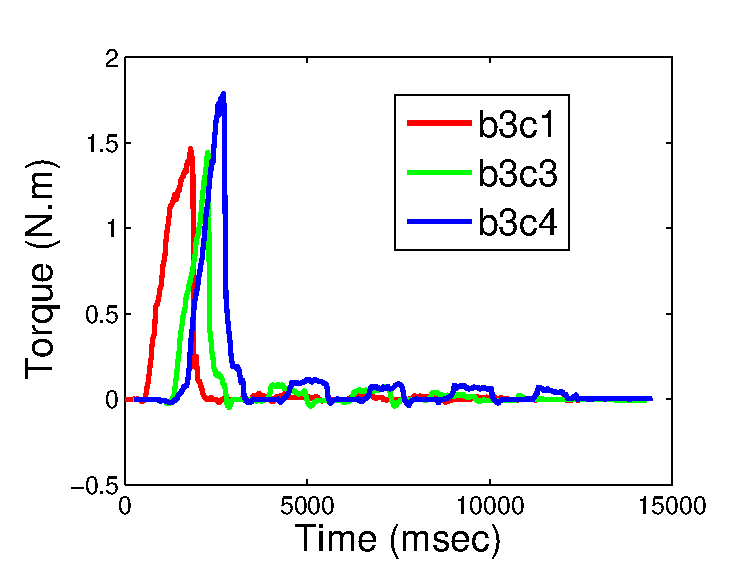
\includegraphics[width=12cm]{./fig_cha4/c1c3c4_time_T.eps}
    \caption{ \scriptsize{Exert torque for opening bottle b3 with three different cap sizes.}
}
\label{fig:cappatterns}
\end{figure}


As mentioned before, the demonstration of each setup is repeated three times and the data from the same setup and same cycle are presumed to belong to the same cluster. To set a threshold for clustering, we check the distances between the time series come from the same setup and the same phase. The largest distance found is 0.04 (normalized) from the $b3c2$ phase 4. We add a $10\%$ margin on this (resulting in 0.044) and use it as the threshold of clustering. The time series distances less than the threshold are grouped into the same cluster. We use the hierarchical agglomerative clustering (Section~\ref{cha4:sec2:learn:cluster}) to merge the data into different clusters. After 5 times of merging, the clusters are not merge-able and 3 clusters remain.

These three clusters contain the data from:

\begin{enumerate}
\item phase I of $b4c3$ (most difficult bottle), 3 time series;
\item phase I of $b3c1, b3c2, b3c3, b3c4, b2c3$ and phase II of $b4c3$, 24 time series;
\item phase I of $b1c3$ (easiest bottle) and phase II of the other setups, 57 time series.
\end{enumerate}

The result of clustering is shown in Table~\ref{tab:cluster}. This result suggests that humans use three different strategies for opening bottles: one for handling the phase I of the most difficult bottle with adhesive materials on the bottle and cap surfaces; one for handling the phase I of most bottles and the phase II of the most difficult bottle; and one for handling the phase I of the lubricated bottle and the phase II of the other bottles. The size of the cap turns out to be playing a less important role in the control strategies. According to this result, we encode these three clusters separately.



%\begin{table*}
%\caption{Clustering results}
%\begin{tabular}{p{1.6cm} p{1.6cm}|p{2cm} p{2cm} p{2cm}  p{2cm} }
%& & \parbox[c]{1em}{\includegraphics[width=1.5cm]{./fig_cha4/c1.jpg}}\newline Cap 1
%& \parbox[c]{1em}{\includegraphics[width=1.5cm]{./fig_cha4/c2.jpg}}\newline Cap 2
%& \parbox[c]{1em}{\includegraphics[width=1.5cm]{./fig_cha4/c3.jpg}}\newline Cap 3
%& \parbox[c]{1em}{\includegraphics[width=1.5cm]{./fig_cha4/c4.jpg}}\newline Cap 4      \\ \hline
%{\parbox[c]{1em}{\includegraphics[width=1.5cm]{./fig_cha4/b1.jpg}}}
%         & Phase I  &           &           & {\vspace{-0.7cm}}\pbox{2cm}{(b1c3) \\ Cluster 3} &           \\
%Bottle 1 & Phase II &           &           &        Cluster 3 &           \\ \hline
%
%{\parbox[c]{1em}{\includegraphics[width=1.5cm]{./fig_cha4/b2.jpg}}}
%%         & Phase I  &{\vspace{-0.7cm}}\pbox{2cm}{(b3c1) \\Cluster 2} &{\vspace{-0.7cm}}\pbox{2cm}{(b3c2) \\Cluster 2} &{\vspace{-0.7cm}}\pbox{2cm}{(b3c3) \\Cluster 2} &{\vspace{-0.7cm}}\pbox{2cm}{(b3c4) \\Cluster 2} \\
%%Bottle 2 & Phase II &       Cluster 3 &       Cluster 3 &       Cluster 3 &       Cluster 3 \\ \hline
%         & Phase I  &           &           &{\vspace{-0.7cm}}\pbox{2cm}{(b2c3) \\Cluster 2} &           \\
%Bottle 2 & Phase II &           &           &       Cluster 3 &           \\ \hline
%
%{\parbox[c]{1em}{\includegraphics[width=1.5cm]{./fig_cha4/b3.jpg}} }
%%         & Phase I  &           &           &{\vspace{-0.7cm}}\pbox{2cm}{(b3c3) \\Cluster 2} &           \\
%%Bottle 3 & Phase II &           &           &       Cluster 3 &           \\ \hline
%         & Phase I  &{\vspace{-0.7cm}}\pbox{2cm}{(b3c1) \\Cluster 2} &{\vspace{-0.7cm}}\pbox{2cm}{(b3c2) \\Cluster 2} &{\vspace{-0.7cm}}\pbox{2cm}{(b3c3) \\Cluster 2} &{\vspace{-0.7cm}}\pbox{2cm}{(b3c4) \\Cluster 2} \\
%Bottle 2 & Phase II &       Cluster 3 &       Cluster 3 &       Cluster 3 &       Cluster 3 \\ \hline
%
%{\parbox[c]{1em}{\includegraphics[width=1.5cm]{./fig_cha4/b4.jpg}}\newline }
%         & Phase I  &           &           &{\vspace{-0.7cm}}\pbox{2cm}{(b4c3) \\Cluster 1} &           \\
%Bootle 4 & Phase II &           &           &       Cluster 2 &           \\ \hline
%\end{tabular}
%\label{tab:cluster}
%\end{table*}

\begin{table*}
\centering
\caption{Clustering results}
\begin{tabular}{p{1.6cm} p{1.6cm}|p{2cm} p{2cm} p{2cm}  p{2cm} }
& & \parbox[c]{1em}{\includegraphics[width=1.5cm]{./fig_cha4/c1.jpg}}\newline Cap 1
& \parbox[c]{1em}{\includegraphics[width=1.5cm]{./fig_cha4/c2.jpg}}\newline Cap 2
& \parbox[c]{1em}{\includegraphics[width=1.5cm]{./fig_cha4/c3.jpg}}\newline Cap 3
& \parbox[c]{1em}{\includegraphics[width=1.5cm]{./fig_cha4/c4.jpg}}\newline Cap 4      \\ \hline
{\parbox[c]{1em}{\includegraphics[width=1.5cm]{./fig_cha4/b1.jpg}}}
         & Phase I  &           &           & {\vspace{-0.7cm}}\pbox{2cm}{(b1c3) \\ Cluster 3} &           \\
Bottle 1 & Phase II &           &           &        Cluster 3 &           \\ \hline
{\parbox[c]{1em}{\includegraphics[width=1.5cm]{./fig_cha4/b2.jpg}}}
%         & Phase I  &{\vspace{-0.7cm}}\pbox{2cm}{(b2c1) \\Cluster 2} &{\vspace{-0.7cm}}\pbox{2cm}{(b2c2) \\Cluster 2} &{\vspace{-0.7cm}}\pbox{2cm}{(b2c3) \\Cluster 2} &{\vspace{-0.7cm}}\pbox{2cm}{(b2c4) \\Cluster 2} \\
%Bottle 2 & Phase II &       Cluster 3 &       Cluster 3 &       Cluster 3 &       Cluster 3 \\ \hline
         & Phase I  &           &           &{\vspace{-0.7cm}}\pbox{2cm}{(b2c3) \\Cluster 2} &           \\
Bottle 2 & Phase II &           &           &       Cluster 3 &           \\ \hline
{\parbox[c]{1em}{\includegraphics[width=1.5cm]{./fig_cha4/b3.jpg}} }
%         & Phase I  &           &           &{\vspace{-0.7cm}}\pbox{2cm}{(b3c3) \\Cluster 2} &           \\
%Bottle 3 & Phase II &           &           &       Cluster 3 &           \\ \hline
         & Phase I  &{\vspace{-0.7cm}}\pbox{2cm}{(b3c1) \\Cluster 2} &{\vspace{-0.7cm}}\pbox{2cm}{(b3c2) \\Cluster 2} &{\vspace{-0.7cm}}\pbox{2cm}{(b3c3) \\Cluster 2} &{\vspace{-0.7cm}}\pbox{2cm}{(b3c4) \\Cluster 2} \\
Bottle 3 & Phase II &       Cluster 3 &       Cluster 3 &       Cluster 3 &       Cluster 3 \\ \hline
{\parbox[c]{1em}{\includegraphics[width=1.5cm]{./fig_cha4/b4.jpg}}\newline }
         & Phase I  &           &           &{\vspace{-0.7cm}}\pbox{2cm}{(b4c3) \\Cluster 1} &           \\
Bootle 4 & Phase II &           &           &       Cluster 2 &           \\ \hline
\end{tabular}
\label{tab:cluster}
\end{table*}



\subsubsection{Learning Modules}
\label{cha4:sec3:learning:module}
We encode the data in each of the modules using GMM. As explained in Section~\ref{cha4:sec2:learn}, a forward model and an inverse model are built for each module. The forward model is encoded by the joint distribution $p\{s(t),s(t-1),a(t-1)\mid\Omega_F\}$, while the inverse model is encoded by $p\{s(t),s(t+1),a(t),a(t-1)\mid\Omega_I\}$. For each model, the number of Gaussians is determined by the BIC. We use 25 Gaussians for cluster 1, 40 for cluster 2 and 15 for cluster 3. Their BIC tests are shown in Fig~\ref{fig:bic}.

\begin{figure}
  \centering
  \includegraphics[width=6cm]{./fig_cha4/bic_cluster1.eps}
  \includegraphics[width=6cm]{./fig_cha4/bic_cluster2.eps}
  \includegraphics[width=6cm]{./fig_cha4/bic_cluster3.eps}
  \caption{ \scriptsize{BIC test result for clusters. (a) Cluster 1, (b) Cluster 2, (c) Cluster 3.}
}

\label{fig:bic}
\end{figure}

%\begin{table}
%\centering
%\renewcommand{\arraystretch}{1.5}
%    \begin{tabular}
%    %{|>{\centering\arraybackslash}p{2cm}|>{\centering\arraybackslash}p{1.2cm}|>{\centering\arraybackslash}p{1.7cm}|>{\centering\arraybackslash}p{1.2cm}|>{\centering\arraybackslash}p{1.5cm}|>{\centering\arraybackslash}p{1.5cm}|>{\centering\arraybackslash}p{1.7cm}|>{\centering\arraybackslash}p{1.7cm}|>{\centering\arraybackslash}p{0.9cm}|}
%    { | c | c | c | c | c |}
%    \hline
%    Cluster & Forward Model &  Inverse Model \\ \hline
%    1       & 98.1\%  & 13.8     \\ \hline
%    2             & 92.1\%  & 21.9    \\ \hline
%    3              & 91.0\%  & 16.0    \\ \hline
%    \end{tabular}
%\caption{Number of Gaussians in each GMM}
%\label{tab:GMM}
%\end{table}


\subsection{Generating motor commands for manipulation}
\label{cha4:sec3:command}
%\label{sec:command}
Our approach is independent of the robot system and can potentially be applied to any robot. We chose to implement this work with a Barrett hand mounted on a KUKA lightweight robot as they are available in our lab. We implemented the multiple module system on this platform to enable the robot to open bottle caps.

\begin{algorithm}
  \caption{Control Algorithm}
  \begin{algorithmic}[1]
    \For{r = 1:4}
    \State REACHING(): Robot moves to initial position\;
        \Function{TURNING()}{} %      \Comment{$\oplus$: bit}
          \State Read previous sensor information $\{s_{t-1},\tau_{t-1},F_{t-1}\}$\;
          \For{k=1:3}
            \State $\hat{s}^{k}$ = FORWARD($s_{t-1},T_{t-1},\Omega_I^k$) \;
          \EndFor
          \For{k=1:3}
            \State $\lambda{k}$ = ResponsibilityFactor($\hat{s}^{k},s_t$) \;
          \EndFor
          \State Read current sensor information $\{s_{t}\}$\;
          \For{k=1:3}
            \State $\{a^k\}$ = INVERSE($s*_{t+1},s_t,a_{t-1}$) \;
          \EndFor
          \State $\{a_t\} = \sum_{k=1,2,3}\lambda{k}\{a^k\}$\;\;
          \State Add compensational torque to $\tau_t$\;
          \State Execute motor command $\{a_t\}$ \;
          \State RELEASING(): Release the cap;
        \EndFunction
    \EndFor

    \While{LIFTCAP() is false}
        \State REACHING();
        \State TURNING();
        \State RELEASING();
    \EndWhile

  \end{algorithmic}
  \label{code:control}
\end{algorithm}


In this experiment, we control the wrist joint (last joint of KUKA) for producing torque to turn the bottle cap. A force torque sensor is fixed under the bottle to provide torque feedback. Each finger of the Barrett hand is mounted with a $Syntouch$\footnote{http://www.syntouchllc.com/} tactile sensor, which is calibrated to provide contact force information, for the grip force feedback. The cap displacement is measured by the wrist joint displacement, assuming that there is no slip between the fingers and the cap.

The target bottle is fixed on the top of a table with it's cap tightened. The robot is placed above it at a distance that allows a proper grasp on the cap. The Barrett hand then close the fingers until the bottle cap is touched. This position is recorded as the initial position, where the cap displacement is marked as zero. In the experiment we focus on the turning cycle. The releasing and reaching cycles are programmed by opening the fingers and restoring to the initial position.

We first test the model with the trained bottles and then test with two new bottles. With each bottle, the turning-releasing-restoring cycles are repeated four times. Data streams from the sensors are filtered to $100Hz$. Once the turning cycle starts, the forward models take the torque and displacement at the last time step as input, and compute the expected displacement of the current time step. These expected displacements are compared with the actual displacement measured at the sensor to evaluate the reliability, expressed as a normalized responsibility factor, of each module. The inverse models take the current displacement, desired next displacement and the previous force and torque as input to compute the proper action (force and torque) to take on the cap. Each of the three outputs is multiplied with its responsibility factor, and the final output is the sum of the factorized three outputs (Algorithm~\ref{code:control}).

In implementation on a real robot, we found that without putting any restriction of the responsibility factor, it can change rapidly. This is caused by the environmental noise in the sensory input and results in instability of the control system. We apply a low pass filter on the responsibility factor to reduce the fluctuation. This filtering implies that the real dynamics does not switch with high frequency, which is consistent with the character of our task.


Before applying the final output on the robot, a compensational torque is added to it in order to compensate the lag causing by the distortion of the robot hand during turning. The control algorithm described above is shown in algorithm~\ref{code:control}.



\subsection{Experiment results}
\label{cha4:sec3:result}

% TODO:
% 1) explain whether the use of the clusters correspond to your expectations and really relate to an identification of different phases
% 2) what the novel object consist of, in what do they differ from the other objects
% 3) what were your expectations in terms of cluster use for these new objects
% 4) Do the results match your expectations

%We implement this algorithm with two bottles (b1 and b4) in the training set and then two bottles (b5 and b6) had not been used for training.
We validated the algorithm to control cap opening in our robot. We first tested the ability of the system to open 2 of the bottles seen during training (b1 and b4). We then tested the generalization capacity of the system by opening two bottles (b5 and b6) not seen during training.
Bottle b1 and b4 are the easiest and most difficult bottles to open in the training set.
Bottle b5 is a large bottle, which is hard for a human to grab and open. Bottle b6 is a glass bottle with a plastic cap. The surface interaction between these two materials is not demonstrated. As the Barrett hand is significantly larger than a human hand, $b1, b4, b6$ are mounted with $c5$ (the cap of $b5$ with diameter $110 mm$) on the top to ensure a firm grasp. In total 4 different setups are used in the experiment: $b1c5, b4c5, b5c5$ and $b6c5$. As discussed above, the size of the cap has minor effect on the control strategy. Therefore we expect the setups $b1c5$ and $b4c5$ will result in a similar behaviour as those of $b1c3$ and $b4c3$ in the training. The experimental results and demonstration snapshots are shown in figures~\ref{fig:demo_b1}-~\ref{fig:demo_b6}~\footnote{Demonstration
  videos are available at http://www.cs.bath.ac.uk/~bh325/opencap.rar}.Figure~\ref{fig:demo_b1b4b5b6} is a similar plot to figure~\ref{fig:bottlepatterns}, that aligns the exerted torque of the 4 experiments.

In each experiment we record the cap displacement, exerted torque, and the responsibility factors of all three modules. Bottle b1 is the easiest bottle to open in the training set, the control policies of both phase $I$ and phase $II$ are grouped into cluster 3. As a result, in the b1 experiment the cluster 3 takes most responsibility (Fig.~\ref{fig:demo_b1}).

Bottle b4 is the most difficult bottle to open in the training set and it's phase $I$ requires more than 3 $Nm$ (Fig.~\ref{fig:bottlepatterns}). Due to the smooth contact surfaces between the Barrett hand and the cap, it is difficult to apply 3 $Nm$ torque to the cap without slipping. To avoid damaging the robot, we test the b4 phase $II$ only: the cap is loosely screwed on the bottle. Without knowing this, in the experiment the robot is able to properly estimate the current task context. As can be seen from the figure~\ref{fig:demo_b4}, different from b1, the dominant cluster is the cluster 2 which corresponds to the b4 phase II. This performance would be hard to achieve by a deterministic system based on expected values for friction coefficients.

Bottle b5 is a novel one but is made of similar material (plastic) to the trained bottles. A very similar torque profile to b2 and b3 is generated for b5: phase $I$ is sharp, while phase $II$ is flattened and significantly smaller than phase $I$ (b2: Fig.~\ref{fig:bottlepatterns}, b3: Fig.~\ref{fig:cappatterns}, b5: Fig.~\ref{fig:demo_b5}). This is because b5 has a dry contact surface as does b2 and b3, whilst b1 is lubricated and b4 is attached with sticky material, i.e. honey.

Bottle b6 is also a novel one but with novel surface materials (plastic and glass). A common way of measuring the FCO of a material is measuring it against metal: the static FCO between glass and metal is 0.5-0.7, while between two polythene and steel is around 0.2. This implies that the plastic and glass are indeed very different in FCO. There is not a universal measurement of the FOC between plastic and glass. It's torque profile is different from what we observed in training the set. Despite this, b6 is opened with the torque profile generated by the three learned modules.
% TODO: Appendix of friction coefficient.

With the above four different setups, the modular model adapts accordingly and successfully generates torque commands to open the bottles. Successful cap opening is achieve when the cap is unscrewed far enough that it can be lifted up. Though no prior information is provided about the bottles, the task contexts are properly estimated and ``contextized'' motor commands are generated to unscrew the caps. These experiments show that our multiple modular approach is indeed effective in manipulation tasks.



\begin{figure*}
  \centering
  \vspace{0.8cm}
  \subfloat[\scriptsize{Snapshots from the robot opening bottle~ $b1$}]
  {\includegraphics[width=13cm]{./fig_cha4/demo_b1.jpg}}

  \vspace{0.3cm}
  %\hspace{0.2cm}
  \subfloat[\scriptsize{Cap displacement during the robot's opening}]
  {\includegraphics[width=13cm]{./fig_cha4/demo_b1_s.eps}}

  \vspace{0.3cm}
  \hspace{-0.3cm}
  \subfloat[\scriptsize{Torque exerted by the robot against cap displacement}]
  {\includegraphics[width=13cm]{./fig_cha4/demo_b1_T.eps}}

  \vspace{0.3cm}
  %\vspace{0.5cm}
  \subfloat[\scriptsize{Responsibility factor against cap
    displacement, for each module}]
  {\includegraphics[width=13cm]{./fig_cha4/demo_b1_rf.eps}}
  \caption{ \scriptsize{The robot opens bottle~$b1$.}
}

\label{fig:demo_b1}
\end{figure*}

\begin{figure*}
  \centering
  \vspace{0.8cm}
  \subfloat[\scriptsize{Snapshots from the robot opening bottle~$b4$}]
  {\includegraphics[width=13cm]{./fig_cha4/demo_b4.jpg}}

  \vspace{0.3cm}
  %\vspace{0.5cm}
  \subfloat[\scriptsize{Cap displacement during the robot's opening}]
  {\includegraphics[width=13cm]{./fig_cha4/demo_b4_s.eps}}

  \vspace{0.3cm}
  \hspace{-0.2cm}
  \subfloat[\scriptsize{Torque exerted by the robot against cap displacement}]
  {\includegraphics[width=13cm]{./fig_cha4/demo_b4_T.eps}}

  \vspace{0.3cm}
  %\vspace{0.5cm}
  \subfloat[\scriptsize{Responsibility factor against cap displacement, for each module}]
  {\includegraphics[width=13cm]{./fig_cha4/demo_b4_rf.eps}}

  \caption{ \scriptsize{The robot opens bottle~$b4$}
}
\label{fig:demo_b4}
\end{figure*}

%JJB --- fix the captions for the below as I already did for the
%above. %JJB
\begin{figure*}
  \centering
  \vspace{0.8cm}
  \subfloat[\scriptsize{Snapshots for robot opening bottle~b5 demonstration}]
  {\includegraphics[width=13cm]{./fig_cha4/demo_b5.jpg}}

  \vspace{0.3cm}
  %\vspace{0.5cm}
  \subfloat[\scriptsize{Cap displacement during the robot's opening}]
  {\includegraphics[width=13cm]{./fig_cha4/demo_b5_s.eps}}

  \vspace{0.3cm}
  %\vspace{0.5cm}
  \subfloat[\scriptsize{Torque exerted by the robot against cap displacement}]
  {\includegraphics[width=13cm]{./fig_cha4/demo_b5_T.eps}}

  \vspace{0.3cm}
  %\vspace{0.5cm}
  \subfloat[\scriptsize{Responsibility factor against cap     displacement, for each module}]
  {\includegraphics[width=13cm]{./fig_cha4/demo_b5_rf.eps}}

  \caption{ \scriptsize{The robot opens bottle~$b5$}
}
\vspace{5cm}
\label{fig:demo_b5}
\end{figure*}

\begin{figure*}
  \centering
  \vspace{0.8cm}
  \subfloat[\scriptsize{Snapshots for robot opening bottle~b6 demonstration}]
  {\includegraphics[width=13cm]{./fig_cha4/demo_b6.jpg}}

  \vspace{0.3cm}
  %\vspace{0.5cm}
  \subfloat[\scriptsize{Cap displacement during the robot's opening}]
  {\includegraphics[width=13cm]{./fig_cha4/demo_b6_s.eps}}

  \vspace{0.3cm}
  \hspace{-0.5cm}
  \subfloat[\scriptsize{Torque exerted by the robot against cap displacement}]
  {\includegraphics[width=13cm]{./fig_cha4/demo_b6_T.eps}}

  \vspace{0.3cm}
  %\vspace{0.5cm}
  \subfloat[\scriptsize{Responsibility factor against cap     displacement, for each module}]
  {\includegraphics[width=13cm]{./fig_cha4/demo_b6_rf.eps}}

  \caption{ \scriptsize{The robot opens bottle~$b6$}
}
\label{fig:demo_b6}
\end{figure*}


\begin{figure}
  \centering
  \includegraphics[width=8cm]{./fig_cha4/rb1b4b5b6_time_T.eps}
  \caption{ \scriptsize{Robot exerted torque for opening four bottles: b1 b4 b5 b6. Time is warped and shifted for displace purpose}
}
\label{fig:demo_b1b4b5b6}
\end{figure}




\section{Discussion}
\label{cha4:sec4}

In this chapter we have presented a modular approach for learning
manipulation tasks from human demonstration. We discover the number of
modules needed in a task by hierarchical clustering. From each cluster
we use forward and inverse model pairs to model the motor control
mechanism. The forward models predict the effect of the previous motor
command, while the inverse models compute a motor command to bring the
current state to a desired state. The statistical approach enables us
to estimate the reliability of the inferences of each module under the
current task context. The final motor command is the sum of the weighted
commands generated by each module. By exploiting an object-centric
viewpoint, the learnt human internal models can be easily transferred
to a robot. Our experiments verify that by this modular approach, the
robot can automatically recognize the current task context and compute
proper motor commands to accomplish a manipulation task, here opening
bottle caps.


Our approach is applicable to manipulation tasks that require adaptive
control strategies. It has a number of benefits compared to existing,
pervasive methods for adaptive control such as classic model
identification adaptive control and reinforcement
learning~\citep{narendra1995adaptation,khalil2004modeling,buchli2011learning}. Because we imitate human behaviors, we do not need to derive the
system dynamics nor the cost function of the tasks, which involve deep
insight into the task and can be painstaking. The difficulty of
modeling an adaptive strategy is further reduced by a modular
approach: dividing the large state space into several subspaces, where
the local strategies can be approximated more accurately. With this
approach, we divide a complex human strategy into a few modules, and
combine them to generate contextualized motor commands.

Our object-centric approach is a practical approach for teaching a
robot manipulation tasks that require proprioception. This allows
human demonstration of the task with physical contact with the object,
which means the demonstrator can have direct feedback from their own
senses and perform the task naturally. We bypass the problem of direct
mapping of human movement and degrees of freedom to a robot's by
expressing the strategy from an object-centric viewpoint. This can
largely benefit learning manipulation tasks such as impedance control
task, as measuring human muscle impedance is hard while measuring the
impedance of an object is more feasible. This approach focus on imitating object movement rather than human movement. For generating natural looking manipulation strategies, however, the object-centric approach does not guarantee good results.

We compute the final motor command by summing the weighted output of
each module. This makes an assumption that the state space is
continuous. For tasks with discontinuous space, switching between different modules would be more applicable~\citep{narendra1995adaptation,nakanishi2013spatio}.

There are many promising directions of further studies extending the
work presented here. The first is to apply this approach to other
contact tasks and learn a more general human control strategy in
handling the instability caused by friction.
%Clarify the fact here that you hardly analyze the effect of changing the cap size and the positioning of the fingers on the cap which is revealed in the tactile signature, and that this will be future work.
In our study, we have focussed on the control strategy of unscrewing
the cap. We hardly analyzed the effect of changing the cap size and or
the positioning of the fingers on the cap, which is revealed in the
tactile signature. For the task here, these were not important and
did not cluster separately, but for other contexts these could be
important. We expect this analysis to advance the study of the task specific grasping
strategy~\citep{el2013generation,dang2014semantic} from the force prospective.

To extend our approach to learn tasks involving multiple steps, one
could also integrate this framework with task segmentation techniques,
to break down the task into atomic steps and recognize the steps
needed, still using an modular approach. However, we could expect this
to complicate the pint of module integration and require
better-informed action selection. 

In summary, tasks involving multiple phases or different contexts are
hard to implement by a single model. A modular architecture is a
practical approach for both learning and controlling these tasks. As
manipulation usually involves multi-phase friction and multi-body
interaction, learning manipulation tasks with a modular approach can
simplify the modeling problem to a significant extent. We have
presented here a framework for training a modular model on observed
human demonstrations, discovering the strategies used by the humans
through a system of cluster analysis, and encoding
the results in generative models capable of driving robots. We have
demonstrated that we can use this framework to transfer strategies
used by a human to a robot, using the task of bottle-cap
opening. The demonstration showed not only `simple' transference from
human to robot, but the capacity for generalizing to similar but
previously-unobserved contexts, and to adapt sequences of actions in
response to the current context.


%%TODO: Modularity comes from... benefit

